\section{Fundamentos de Mapas Geográficos}
	
	\subsection{Coordenadas}
	Coordenadas são usadas para expressar localizações no mundo. Existem vários sistemas de coordenadas diferentes. O usado pelo Google Maps é o Word Geodetic System 84 (WGS84), que é o mesmo sistema que o Global Position System(GPS) usa. As coordenadas são expressas usando o conceito de latitude e longitude. Onde latitude mede do sul ao norte e longitude me do oeste para o leste. No equador a latitude é 0. Isso significa que tudo abaixo do equador (hemisfério sul) possui uma latitude negativa, e tudo acima possui uma latitude positiva. Similarmente também existe uma linha zero para longitude. É conhecida como meridiano, e por razões históricas passa por Greenwich, Inglaterra. Cada posição que é localizada a leste desta linha tem um número positivo e tudo a oeste tem um número negativo\cite[4]{livroGoogleApiV3}. 
	
	A \autoref{fig-coordenadas} permite uma melhor observação desses conceitos:
	\begin{figure}[htb]
	\caption{\label{fig-coordenadas} O centro do mundo na latitude 0 e longitude 0 reside em algum lugar a oeste da costa da África}
	\begin{center}
	    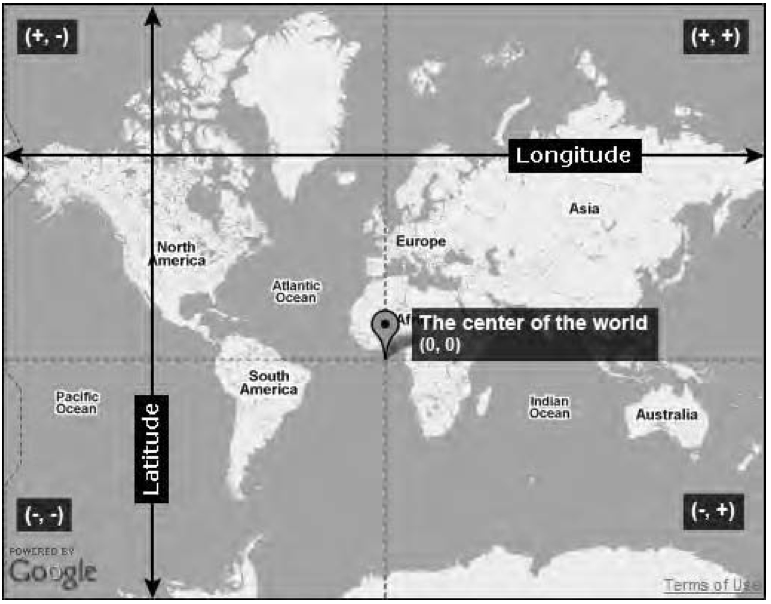
\includegraphics[scale=0.4]{goo-coordenadas}
	\end{center}
	\legend{Fonte: \cite[5]{livroGoogleApiV3}}
	\end{figure}
	
	
	Dessa forma é possível representar o mapa do mundo em uma imagem retangular projetada sobre o plano cartesiano. 
	
	\subsection{Marcadores e Icones} pag 140
	\subsection{InfoWindow} videos e fotos pagina 152
	\subsection{Polylines}

\section{Estratégias para lidar com muitos marcadores}
  \subsection{Reduzir numero de marcadores}
	\subsubsection{Pesquisa}
	\subsubsection{Filtro}
	\subsubsection{Otimizar a representação}
nem sempre usar marcadores para representar cada parte de um elemento... linhas nao precisam de marcadores para cada vertice , e grupos proximos podem de ser representados por unico poligono.
 pagina 198
 LEIA:
 
 (pagina 88 ,silva, tabela 6, figura 93, figura 65 ())

  \subsection{Agrupamento/Clustering}
  pagina 199 (google)
		\subsubsection{Por grelha}
		\subsubsection{Por distancia}
		\subsubsection{Por região}
		
\section{Algorítimos de agrupamento}
	\subsection{Métodos baseados em grelha}
		\subsubsection{WaveCluster}
	\subsection{Aplicações}
		\subsubsection{MarkerCluster}
		pagina 206 a 212
		\subsubsection{MarkerClustered}



\section{Planilhas eletrônicas e Mapas}
\subsection{O desafio chinês}
mostra o uso de planilhas pelo governo chines \cite{chinaPlanilha}
\subsection{Domínios de conhecimento}
Mostra a importância do uso de planilhas \cite{credinePlanilha} 
\subsection{Usando planilhas como fonte de dados para Mapas Geográficos}
Mostra \cite{lieberman2009spatio}